\documentclass{数学建模}


\begin{document}
\renewcommand{\thesubsection}{\thesection.\arabic{subsection}}
\renewcommand{\thesubsubsection}{\thesubsection.\arabic{subsubsection}}



% \vspace*{\fill}

% \noindent\heiti \zihao{-3}报名序号:1436

% \vspace{3cm}
% \noindent\heiti \zihao{-3}赛题题目:电采暖负荷参与电力系统功率调节的技术经济分析

% \raggedbottom
% \vspace*{\fill}

% \newpage



\songti \zihao{-4}
\begin{center}
    {\heiti \zihao{-3}\textbf{塔式光热电站镜场光学效率计算及输出热功率优化设计}}
\end{center}

\begin{center}
    {\heiti \zihao{-3}\textbf{摘要}}
\end{center}

本文在求定日镜光学效率及单位镜面面积年平均输出热功率的设计中,
通过光反射分析,建立了太阳光、定日镜和集热器光反射-接收模型,
并使用蒙特卡罗光线追踪法和Möller–Trumbore算法结合,同时建立镜面
坐标系并求出与地面坐标系之间的转换矩阵,求解出阴影遮挡、集热截
断效率等参数。在此基础上,通过粒子群-遗传混合算法及自适应引力搜
索算法,求出了最大单位镜面面积年平均输出热功率和相应的吸收塔位置
坐标、定日镜尺寸、定日镜数目等参数,并对模型进行了检验和误差分析。

\textbf{针对问题一:}首先,基于对坐标系灵活选取,建立了定日镜-集热器
光线模型。其次,建立了镜面坐标系,推导出其与地面坐标系之间的转换矩阵
。最后,使用蒙特卡洛光线追踪法和离散化镜面法,结合Möller–Trumbore算法
求解出阴影遮挡效率和截断效率,进行求解出平均光学效率。得到了1月21日
平均光学效率为0.6535332,平均余弦效率为0.7649707,平均阴影遮挡效率为0.9847608,平均截断效率
为0.9751661,单位平均输出热功率为0.6992664。结果详细见文中表2和表3。

\textbf{针对问题二:}在上述定日镜-集热器光线模型和坐标系转换的基础上,
由于塔的坐标移动会大大提高数据量,因而我们进行分步,先在大圆上确定定日镜
排布,再用一小圆移动坐标系确定吸收塔位置,最后计算最优解。首先建立大圆的
坐标系,然后使用粒子群-遗传混合算法及自适应引力搜索算法,求解出定日镜的
最优排布,和镜子的最优尺寸然后我们再在x轴上移动半径为350m的真圆,搜索最
大化目标函数的圆心位置,即吸收塔的位置。得到了单位镜面面积年平均输出热功
率为0.6690383166。结果详细见表1、表2、表3及result2.xlsx文件。

\textbf{针对问题三:}与第二问类似,新增要求每片镜子的尺寸,如果逐一进行
计算会过于复杂,因此,我们通过聚类方法将定日镜分为几类,每类的尺寸相同,
在此过程中,与第二问类似,使用粒子群-遗传混合算法及自适应引力搜索算法优化
定日镜排布。通过多重聚类的方法定义聚类目标函数,为每一类定日镜定义一个聚类
目标函数。使用k-means聚类算法来求解每一类定日镜的尺寸和高度以及位置和
吸收塔的位置坐标。结果详细见表1、
表2、表3及result3.xlsx。

\noindent \zihao{-4}\textbf{ 关键字:} 塔式光热电站镜场; 光学效率; 
平均输出热功率; 蒙特卡洛光线追踪法; 粒子群-遗传混合算法; k-means聚类算法

\newpage

\section{问题重述}
\subsection{问题的背景}

塔式太阳能光热发电是一种低碳环保的新型清洁能
源技术。但是定日镜场子系统与塔式光热电站的综合性能有着密
切的关系,是塔式光热电站的关键子系统之一。镜
场中的定日镜数目众多,而电站一旦建成定日镜的
位置就无法修改,因此定日镜场的光学效率计算问
题与优化布置理论显得至关重要。


\subsection{问题的重述}

\textbf{装置结构:}
塔式太阳能光热发电站由定日镜、吸收塔、集热器组成。定日镜
由底座和平面反射镜构成,底座由纵向和水平转轴组成,可以控制
反射镜的方向,集热器位于镜场中吸收塔的顶端。

\textbf{工作原理:}
塔式电站由大量的定日镜组成阵列,定日镜将太阳光反射汇聚
到安装在镜场中吸收塔顶端的集热器中,加热其中的导热介质,
并将太阳能以热能形式储存起来,经热交换实现由热能向电能
的转化。

\textbf{问题一:}
已知吸收塔建于该圆形定日场中心,定日镜为6m*6m,安装高度均为
4m,并已知所有定日镜位置。求1-12月每个月平均余弦效率、平均
阴影遮挡效率、平均截断效率,平均光学效率、单位面积镜面平均
输出热功率以及年平均各项参数值。

\textbf{问题二:}
目标要使单位镜面面积年平均输出热功率最大,已知所有定日镜尺寸
及安装高度相同,定日镜数目、位置、尺寸、高度以及吸收塔的位置
均未知。约束限定定日镜场的额定年平均输出热功率为60MW,安装高度
在2m至6m之间,镜面边长在2m至8m之间,且相邻底座中心之间的距离
比镜面宽度多5m。

\textbf{问题三:}
在第二问的基础上,需要重新设计定日镜场的各个参数,以满足额
定功率的条件,并使单位镜面面积年平均输出热功率尽量大。

\section{问题分析}

\subsection{问题一的分析}
问题一首先需要建立定日镜-集热器光线模型,
本小问难点在于准确计算阴影遮挡效率等光学效率参数。
对此,灵活选取坐标系,在镜场坐标系中引入镜面坐标系,
推导出两者之间的转换矩阵。同时使用蒙特卡罗光线追踪
法,离散化定日镜的表面,等效计算每个点上计算光线效率。
然后使用Möller–Trumbore算法结合上述基础,求解出阴影
遮挡效率和截断效率以及其他光学效率参数。

\subsection{问题二的分析}

在问题一的基础上,在定日镜参数未定的情况下,需要求出单位镜面面积年平均输出热功率
尽可能大。本小问分两步进行求解,第一步通过粒子群-遗传混合算法和引力搜索优化法求
出最优定光镜排布和尺寸,第二步通过坐标系移动求出接收塔最佳位置。


\subsection{问题三的分析}

在问题二的基础上,由于定日镜尺寸不同、高度也不同,需要进一步
考虑以单位镜面面积年平均输出热功率最大为目标的优化函数模型,
通过多重聚类的方法定义聚类目标函数,最后使用k-means聚类算法来
求解每一类定日镜的尺寸和高度以及位置和吸收塔的位置坐标。

\section{模型假设}
为了适当地对模型进行合理化简化,本文给出如下假设:

1、假设吸收塔的直径与集热器直径相同且上下柱体相同均为7米。

2、假设每月21日均为晴天,不考虑阴雨等天气对数据的影响。

3、假设所有平面镜完好且不考虑平面镜上灰尘等影响。

\section{符号说明}
\begin{center}
    \begin{longtable}{|c|>{\centering\arraybackslash}p{8cm}|c|}
        \hline
        符号 & 含义 & 单位  \\
        \hline
        $\alpha_s$ & 太阳高度角 & $^\circ$ \\
        \hline
        $\gamma_s$ & 太阳方位角 & $^\circ$ \\
        \hline
        $\varphi $ & 当地纬度 &  $^\circ$\\
        \hline
        $\omega $ & 太阳时角 &  $^\circ$ \\
        \hline
        $\delta $ & 太阳赤纬角 & $^\circ$ \\
        \hline
        $ST$ & 当地时间 & - \\
        \hline
        $D$ & 计算天数 & -\\
        \hline
        $DNI$ & 法向直接辐射辐照度 & $kw/m^2$ \\
        \hline
        $H$ & 海拔高度 & $km$ \\
        \hline
        $G_s$ & 太阳常数 & $kw/m^2$ \\
        \hline
        $\eta $ & 光学效率 & - \\
        \hline
        $E_{field}$ & 定日镜场输出热功率 & $kw$ \\
        \hline
        $N$ & 定日镜总数 & 面 \\
        \hline
        $A_i$ & 第i面定日镜采光面积 & $m^2$ \\
        \hline
        $\eta _i$ & 第i面镜子的光学效率 & - \\
        \hline
        $\eta _{sb}$ & 阴影遮挡效率 & - \\
        \hline
        $\eta _{cos}$ & 余弦效率 & - \\
        \hline
        $\eta _{at}$ & 大气透射率 & - \\
        \hline
        $\eta _{trunc}$ & 余弦效率 & - \\
        \hline
        $\eta _{ref}$ & 镜面反射率 & - \\
        \hline
        $d_{HR}$ & 镜面中心到集热器中心的距离 & $m$ \\
        \hline
    \end{longtable}
    \label{tab:example}
\end{center}



\section{模型的建立与求解}

% \begin{figure}[H]  
%     \centering\includegraphics[width=0.8\linewidth]{绘图1.jpg}  
%     \caption{模型建立思路流程图}     
%     \label{img01}   
% \end{figure}

% 此图最主要的特点是在常规求解等值模型常微分方程的基础上,在温度控制
% 范围内,使用SIR模型和离散欧拉法进行求解数值解,这样的优点能够较快
% 的求解出常微分方程,并且通过上述两种方法可以提高预测的精度。之所以
% 使用这种方法的原因在于,原方程参数较多,不易直接求解,需转化形式为
% 差分方程获迭代格式求解较为方便。

\subsection{问题一模型的建立与求解}
\subsubsection{镜面坐标系的建立与转换}
由于在计算光学效率的过程中,需要建立镜面坐标系
与镜场坐标系进行转换
设有一个镜场坐标系下的向量:
\begin{equation}
    \overrightarrow{a} = (\overrightarrow{i},\overrightarrow{j},\overrightarrow{k})
\end{equation}

在镜面坐标系下为:
\begin{equation}
    \overrightarrow{b} = (\overrightarrow{i_i},\overrightarrow{j_i},\overrightarrow{k_i})
\end{equation}



\begin{equation}
    P_i = \begin{pmatrix}
        \overrightarrow{i_{i_x}} & \overrightarrow{j_{i_x}} & \overrightarrow{en_{i_x}} \\
        \overrightarrow{i_{i_y}}& \overrightarrow{j_{i_y}} & \overrightarrow{en_{i_y}} \\
            0 & \overrightarrow{j_{i_z}} & \overrightarrow{en_{i_z}} \\
    \end{pmatrix}
\end{equation}

经推导可得镜面坐标系和镜场坐标系存在$ \overrightarrow{b} = \overrightarrow{a} P_i$

且\begin{equation}
    P_i = \begin{pmatrix}
        \overrightarrow{i_{i_x}} & \overrightarrow{j_{i_x}} & \overrightarrow{en_{i_x}} \\
        \overrightarrow{i_{i_y}}& \overrightarrow{j_{i_y}} & \overrightarrow{en_{i_y}} \\
            0 & \overrightarrow{j_{i_z}} & \overrightarrow{en_{i_z}} \\
    \end{pmatrix}
\end{equation}

又因为$(\overrightarrow{en_{i_x}},\overrightarrow{en_{i_y}},\overrightarrow{en_{i_z}}) = 
\overrightarrow{n_i}$,$\overrightarrow{n_i}$为镜面法向量。
且
\begin{equation}
    \overrightarrow{i_i}  \bot \overrightarrow{k_i}
\end{equation}
所以有
\begin{equation}
    \begin{cases}
        \overrightarrow{i_{i_x}} \overrightarrow{en_{i_x}} + \overrightarrow{i_{i_y}} \overrightarrow{en_{i_y}} =0\\
        \overrightarrow{i_{i_x}}^2 + \overrightarrow{i_{i_y}}^2 = 1\\
    \end{cases}
\end{equation}


经过推导可知矩阵$P_i$为一个正交矩阵,所以
\begin{equation}
    P_i^T = P_i ^{-1}
\end{equation}

由此可以推出$ \overrightarrow{a} = P_i^{T} \overrightarrow{b} $

\subsubsection{蒙特卡罗光线追踪法模型建立}
首先定义一个反射方程
\begin{equation}
    L_r(\overrightarrow{x},\overrightarrow{\omega_r}) = \int_\varGamma f_r(\overrightarrow{x},\overrightarrow{\omega_i}\rightarrow \overrightarrow{\omega_r}
    L_i(\overrightarrow{x},\overrightarrow{\omega_i})\cos(\theta_i)d\omega_i)
\end{equation}
经计算,形式解为
\begin{equation}
    L(\overrightarrow{x},\overrightarrow{\omega }  ) = \sum_{i = 0}^{\infty}K^i L_e(\overrightarrow{x_0},\overrightarrow{\omega_0}) 
\end{equation}

\subsubsection{Möller–Trumbore 算法模型}
首先定义一个标量三重积,设$\overrightarrow{a} $,$\overrightarrow{b} $,$\overrightarrow{c} $为三个向量

\begin{equation}
    a\cdot (b\times c) = b\cdot (c\times a) = c\cdot (a\times b) = A
\end{equation}


\begin{equation}
    A = \begin{pmatrix}
        a_{one} & a_{two} & a_{three} \\
        b_{one} & b_{two} & b_{three} \\
        c_{one} & c_{two} & c_{three} \\
    \end{pmatrix}
\end{equation}

任意兑换两个向量的位置,标量三重积与原来相差一个负号:
\begin{equation}
    \begin{cases}
    a\cdot (b\times c) = -a\cdot (c\times b)\\
    a\cdot (b\times c) = -b\cdot (a\times c)\\
    a\cdot (b\times c) = -c\cdot (b\times a)\\
    \end{cases}
\end{equation}

通过克莱姆法则,一个线性方程组可以用矩阵与向量的方程来表示$Ax=c$,如果
A是一个可逆矩阵$(det(A)\neq 0)$,那么方程有解$x=(x_1,x_2,\dots X_n)^T$,
其中$A_i$是被列向量取代了A的第i列的列向量后得到的矩阵。

经过推导可知:
根据克莱姆法则
\begin{equation}
    t = \frac{det[S E_1 E_2]}{det[-d E_1 E_2]} 
\end{equation}

根据三重积
\begin{equation}
    det([S E_1 E_2]) = (S\times E_1)\cdot E_2
\end{equation}

\begin{equation}
    det([-d E_1 E_2]) = -d \cdot (E_1\times E_2) =  E_1\cdot(d\times E_2)
\end{equation}

可以得到
\begin{equation}
    b1 = \frac{det[-d S E_2]}{det[-d E_1 E_2]} = \frac{S_1\cdot S}{S_1\cdot E_1}
\end{equation}

\begin{equation}
    b2 = \frac{det[-d E_1 S ]}{det[-d E_1 E_2]} = \frac{d \cdot (S\times E_2)}{S_1\cdot E_1}
\end{equation}

整理得:
\begin{equation}
    [t,b1,b2 ]^T = \frac{1}{S_1\cdot E_1}  [S_2 \cdot E_2,S_1 \cdot S,S_2 \cdot d ]^T
\end{equation}

\subsubsection{求解过程}

\textbf{1.求解余弦效率:}


已知
\begin{equation}
    \begin{cases}
        x_{i} = cos(\alpha_s)*cos(90^\circ - \gamma_s)  \\
        y_{i} = cos(\alpha_s)*sin(90^\circ - \gamma_s)  \\
        z_{i} = sin(\alpha_s)
    \end{cases}
\end{equation}
假设镜面中心指向集热器中心的向量为$\overrightarrow{AO} $:
\begin{equation}
    \vec{AO} =(0,0,84) -(x_k,y_k,4) = (-x_k,-y_k,80)
\end{equation}
然后对向量$\overrightarrow{AO} $进行单位化:
\begin{equation}
    \vec{b} = \frac{\vec{AO}}{|\vec{AO}|}
\end{equation}
由平行四边形原则可得向量$\vec{n}$,并进行单位化处理:

\begin{equation}
    \vec{n} = \frac{\vec{i} + \vec{b}}{|\vec{i} + \vec{b}|}
\end{equation}

式子中$\vec{n}$为镜面法向量,$\vec{i}$为入射光线反方向的单位向量
,由太阳在地平坐标系中的相对位置来确定。
太阳在地平坐标系中的位置用高度角$\alpha_s $和方位角$\gamma_s$来表示
则入射光线的反方向的单位向量
$\vec{i}$(方向由镜面反射点指向太阳)的表达式为:

\begin{equation}
    \vec{i} = [ \cos (\alpha_s) \sin (\gamma_s),  \cos (\alpha_s) \cos (\gamma_s),  \sin (\alpha_s)] 
\end{equation}
从而可以解得余弦效率为:
\begin{equation}
    \eta_{\cos} = \cos \theta = \vec{i} \cdot \vec{n}
\end{equation}



\textbf{2.求解平均阴影遮挡效率:}


在镜面坐标系下,设每个面的顶点坐标为:
$P_{1_k}=(a_1,b_1,c_1),P_{2_k}=(a_2,b_2,c_2),P_{3_k}=(a_3,b_3,c_3)
,P_{4_k}=(a_4,b_4,c_4)$

由于转换方程需要使用高度角和方位角,
设镜面中心坐标为$O(x_n,y_n,z_n)$,镜子高度为$h$
所以求解俯仰角
\begin{equation}
    \theta_s = \arctan(\frac{\sin (\alpha_s) \cdot m + h_0}{\sqrt{x_{n}^2 + y_{n}^2 + m^2 \cdot \cos ^2(\alpha_s) - 2 \cos (\alpha_s) \cdot m \cdot (x_{n} \cdot \sin (\gamma_s) - y_{n} \cdot \cos (\alpha_s))} } \\
\end{equation}

所以求解方位角
\begin{equation}
    \theta_z = \arcsin (\frac{x_{n} - \cos (\alpha_s) \cdot \sin (\gamma_s) \cdot m}{\sqrt{x_{n}^2 + y_{n}^2 + m^2 \cdot \cos ^2(\alpha_s) - 2 \cos (\alpha_s) \cdot m \cdot (x_{n} \cdot \sin (\gamma_s) - y_{n} \cdot \cos (\alpha_s))} } ))
\end{equation}

其中,$m=\sqrt{x_{n}^2+y_{n}^2+h_{0}^2} $

经过坐标系转换 :
在镜场坐标系下的坐标为
$P_{1_k}=(a_1,b_1,c_1),P_{2_k}=(a_2,b_2,c_2),P_{3_k}=(a_3,b_3,c_3),
P_{4_k}=(a_4,b_4,c_4)$

由于同一个定日镜场中定日镜的尺寸是一样的,设定日镜长度为$l$,同时已知俯仰角$\theta_s$,
和方位角$\theta_z$,得到定日镜四个顶点在镜场坐标系下的坐标

\begin{equation}
    \begin{cases}
        a_1 = x_n + \frac{1}{2}l*cos(\theta_s) -  \frac{1}{2}l*sin(\theta_s) \\
        b_1 = y_n + \frac{1}{2}l*cos(\theta_s) +  \frac{1}{2}l*sin(\theta_s) \\
        c_1 = h_0 + \frac{1}{2}l*sin(\theta_z)  \\
    \end{cases}
\end{equation}

\begin{equation}
    \begin{cases}
        a_2 = x_n - \frac{1}{2}l*cos(\theta_s) -  \frac{1}{2}l*sin(\theta_s) \\
        b_2 = y_n + \frac{1}{2}l*cos(\theta_s) -  \frac{1}{2}l*sin(\theta_s) \\
        c_2 = h_0 + \frac{1}{2}l*sin(\theta_z)  \\
    \end{cases}
\end{equation}

\begin{equation}
    \begin{cases}
        a_3 = x_n - \frac{1}{2}l*cos(\theta_s) +  \frac{1}{2}l*sin(\theta_s) \\
        b_3 = y_n - \frac{1}{2}l*cos(\theta_s) -  \frac{1}{2}l*sin(\theta_s) \\
        c_3 = h_0 - \frac{1}{2}l*sin(\theta_z)  \\
    \end{cases}
\end{equation}

\begin{equation}
    \begin{cases}
        a_4 = x_n + \frac{1}{2}l*cos(\theta_s) +  \frac{1}{2}l*sin(\theta_s) \\
        b_4 = y_n - \frac{1}{2}l*cos(\theta_s) +  \frac{1}{2}l*sin(\theta_s) \\
        c_4 = h_0 - \frac{1}{2}l*sin(\theta_z)  \\
    \end{cases}
\end{equation}

然后使用蒙特卡罗光线追踪法进行离散化镜面处理,将镜面分为
$k*n$个小的方块,取每个小的方块中心点坐标,设每个中心
点为$O_k$,
\begin{equation}
    \overrightarrow{P_{1_k}O_k} = \frac{6}{k} \overrightarrow{P_{1}P_{2}} + \frac{6}{n} \overrightarrow{P_{1}P_{3}}
\end{equation}
得到点$O_k=(x_0,y_0,z_0)$在镜场坐标系中的坐标

同时已知入射方向向量$\vec{i} = [ \cos (\alpha_s) \sin (\gamma_s),  \cos (\alpha_s) \cos (\gamma_s),  \sin (\alpha_s)]$,
得到该直线方程为
\begin{equation}
    \frac{x-x_0}{\cos (\alpha_s) \sin (\gamma_s)} = \frac{y-y_0}{\cos (\alpha_s) \cos (\gamma_s)} = \frac{z-z_0}{\sin (\alpha_s)} = t
\end{equation}
从而可以得到
\begin{equation}
    \begin{cases}
        x = x_0 + \cos (\alpha_s) \sin (\gamma_s) t \\
        y = y_0 + \cos (\alpha_s) \cos (\gamma_s) t \\
        z = z_0 + \sin (\alpha_s) t  \\
    \end{cases}
\end{equation}

然后再求出目标定向镜面的平面方程,设法向量为$\overrightarrow{n} = (A,B,C) $,通过一点镜面中心为$O_s = (x_k,y_k,4)$,
从而解得平面当成为
\begin{equation}
    A(x-x_k)+B(y-y_k)+C(z-z_k)=0
\end{equation}

最后将上述x,y,z带入目标定向镜面的平面方程,从而解得t的值,如果$t>0$,则证明此线与面有交点,即被遮挡,如果$t<=0$,则证明
此线与平面没有交点,即没有被遮挡。同样,阴影情况下相同,只需把入射方向的方向向量换成反射方向的方向向量。最后使用计算及图形学
里面的 Möller–Trumbore 算法进行求解验证。

\textbf{3.求解集热器截断效率:}

求解原理本质与阴影遮挡相同,都是将镜面分割为数小块,
通过已知的入射光线向量与镜面法向量计算出反射法向量,
再判断与集热器是否有交点,如果有交点则证明接收到了
光线,如果没有交点则证明没有接收到光线。

求解反射光线方法与阴影遮挡基本相似,在此不再重复,我们
对集热器做了近似处理,认为集热器是一个长方体,然后
使用图形计算学轻松判别即可。

\textbf{4.求解单位面积镜面平均输出热功率:}

设单位面积镜面平均输出热功率为$Eave_{fiele}$,发光总面积为$M$,由题目已知
定日镜输出热功率为:
\begin{equation}
    E_{field}= DNI\cdot \sum_{i}^{N} A_i \eta_i
\end{equation}
所以:
\begin{equation}
    Eave_{fiele} = \frac{DNI\cdot \sum_{i}^{N} A_i \eta_i}{M}
\end{equation}
其中 DNI 为法向直接辐射辐照度;$N$ 为定日镜总数(单位:面);$A_i$ 为第 $i$ 面定日镜采光面积(单位:m2 ); $\eta_i$ 为第 $i$ 面镜子的光学效率。

\begin{equation}
    DNI = G_0 [a + b \exp(-\frac{c}{\sin \alpha_s})]
\end{equation}

\begin{equation}
    \begin{cases}
        a = 0.4237 - 0.00821(6 - H)^2\\
        b = 0.5055 + 0.00595(6.5 - H)^2 \\
c = 0.2711 + 0.01858(2.5 - H)^2 \\
    \end{cases}
\end{equation}
其中 $G_0$ 为太阳常数,其值取为 1.366 kW/m2 ,H 为海拔高度 (单位:km)
\begin{equation}
    \sin \alpha_s = \cos \varphi \cos \delta \cos \omega + \sin \varphi \sin \delta
\end{equation}


其中太阳方位角为 $\gamma_s$

$$
\cos \gamma_s = \frac{\sin \delta - \sin \alpha_s \sin \varphi}{\cos a_s \cos \varphi}
$$

其中 $\varphi$ 为当地纬度,北纬为正; $\omega$ 为太阳时角

$$
\omega = \frac{\pi}{12} \times (ST - 12)
$$

其中 ST 为当地时间, $\delta$ 为太阳赤纬角[5]

$$
\sin \delta = \sin \frac{2 \pi D}{365} \sin \frac{2 \pi}{360} 23.45
$$

其中 D 为以春分作为第 0 天起算的天数,例如,若春分是 3 月 21 日,则 4 月 1 日对应 D = 11。



\textbf{5.求解大气透射率:}

有题目已知:
\begin{equation}
    \eta_{at} = 0.99321 - 0.0001176d_{HR} + 1.97\times 10^{-8}\times d_{HR}^2(d_{HR}< = 1000)
\end{equation}
其中$d_{HR}$表示镜面中心到集热器中心的距离。

\textbf{6.定日镜的光学效率:}

在上述各个效率已知的情况下:
\begin{equation}
    \eta = \eta_{sb}\eta_{cos}\eta_{at}\eta_{trunc}\eta_{ref}
\end{equation}
求出每个月的平均光学效率及年平均光学效率

\subsubsection{结果分析及验证}
\textbf{1.表一、表二结果如表所示:}

\begin{center}
    \renewcommand{\arraystretch}{1.5}
    \begin{table}[htbp]
        \centering
        \caption{问题一每月21日平均光学效率及输出功率}
        \resizebox{\textwidth}{!}{
          \begin{tabular}{|*{6}{c|}}
            \hline 
            \makecell{日期} & 平均光学效率 & 平均余弦效率 & 平均阴影遮挡效率 & 平均截断效率 & 单位面积镜面平均输出热功率($kw/m^2$) \\
            \hline
            1月21日 &0.6535332008992 &0.7649707361417448 &0.984760834 &0.975166126 &0.6992664  \\
            \hline
            2月21日 &0.6737274939632 &0.7832864364541885 &0.986843987 &0.979722613 &0.6501465  \\
            \hline
            3月21日 &0.6744532067694 &0.7927813457422291 &0.972222965 &0.983604216 &0.6609641  \\
            \hline
            4月21日 &0.6857870629807 &0.7961058452927791 &0.977682325 &0.990420143 &0.6789222  \\
            \hline
            5月21日 &0.6811902190941 &0.7931033121094988 &0.974857263 &0.990482644 &0.6880019  \\
            \hline
            6月21日 &0.6722305512452 &0.782582872076416  &0.980000298 &0.985356811 &0.6587854 \\
            \hline
            7月21日 &0.6384449124169 &0.7646187195458157 &0.955583334 &0.982305589 &0.6654912  \\
            \hline
            8月21日 &0.6184542788866 &0.7412604186524585 &0.947344826 &0.990297226 &0.6635248  \\
            \hline
            9月21日 &0.6208932435781 &0.7209575117008334 &0.984119999 &0.983680421 &0.6712351  \\
            \hline
            10月21日 &0.6057814662874 &0.7131902292611617&0.964054999 &0.990420143 &0.6623156  \\
            \hline
            11月21日 &0.6226907645571 &0.7217189398583448&0.974857564 &0.994892644 &0.6756241  \\
            \hline
            12月21日 &0.6260176006577 &0.7416393073744009&0.960000001 &0.988536811 &0.6543261 \\
            \hline
          \end{tabular}
        }
        \label{tab:example}
      \end{table}
\end{center}

\begin{center}
    \renewcommand{\arraystretch}{1.5}
    \begin{table}[htbp]
        \centering
        \caption{问题一年平均光学效率及输出功率表}
        \resizebox{\textwidth}{!}{
          \begin{tabular}{|*{5}{c|}}
            \hline 
            平均光学效率 & 平均余弦效率 & 平均阴影遮挡效率 & 平均截断效率 & 单位面积镜面平均输出热功率($kw/m^2$) \\
            \hline
            0.647739433 &0.759676213 &0.971745236 &0.986259666 &0.669047733  \\
            \hline
          \end{tabular}
        }
        \label{tab:example}
      \end{table}
\end{center}

\textbf{2.结果分析验证:}
\begin{figure}[H]  
    \centering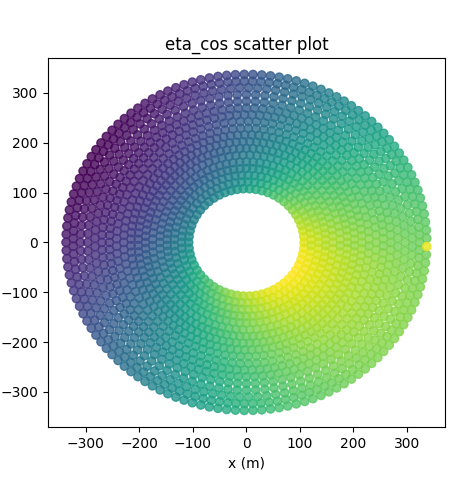
\includegraphics[width=0.7\linewidth]{余弦效率1.png}  
    \caption{余弦效率}     
    \label{img01}  
\end{figure}

如图所示为3月21日9点余弦效率的示意图,可以较为直观的看出,余弦效率的分布情况


\subsection{问题二模型的建立与求解}

\subsubsection{目标函数与约束条件}

问题二是一道优化问题,要求最大化单位镜面面积年平均输出热功率,即MAX目标函数
\begin{equation}
    max w=E_{field}/(N*S)
\end{equation}


同时题目给出了一些约束条件,首先额定年平均输出热功率为60MW,
其次安装高度在2m至6m之间,镜面边长在2m至8m之间,安装高度需使镜面不触地。
最后相邻底座中心之间的距离比镜面宽度多5m。




\subsubsection{问题二模型的建立}

首先,设在一个同心圆环阵列中,辐射场的阵因子为:
\begin{equation}
    F(\theta ,\varphi ) = \sum_{i = 1}^{M} \sum_{l = 1}^{N_i}
    I_{il}e^{j\alpha_{il}}e^{jk\rho_i sin(\theta )cos(\varphi -\varphi_{il})}  
\end{equation}
式中:$M$为圆环数目,$N_i$为第$i$个圆环上振元的个数,$I_{il},\alpha_{il},\varphi_{il}$表示
第i个圆环上第l个阵元的激励幅度及相位角。

由于需要建立一个同心圆阵列的适应度函数,可以根据单位镜面面积输出热功率最大的单目标
,适应度函数可以设置如下:
\begin{equation}
    f_{fit} = [a \cdot |L_m - L_e|^2 + b\cdot |A_m - E_F|^2]^{\frac{1}{2}}
\end{equation}
在以上式子中,$L_m$,$L_e$代表实际方向的最大输出热功率,a,b是加权系数。

然后使用粒子群进行搜索,当第$i$个粒子第$t+1$次迭代时,第m维的速度可以推算出是:

\begin{equation}
    \nu_{i}^m(t+1) = rand_i \cdot \nu_{i}^m(t) + \sum_{j \in k_{best}}^{N} 
    rand_i \cdot G(t)\frac{M_{j}(t)}{R_{ij}(t)+\partial } (x_{j}^m(t) - x_{i}^d(t))  
\end{equation}

然后第一部分是确定定日镜的排布,第二部分是确定吸收塔的位置。
通过建立坐标系,以原点为中心建立一个半径为700的大圆,在大圆中
模拟优化求出定日镜的最佳排布方式,目标是最大化所有定日镜光学
效率之和,

得出大圆的最优镜面拍布后,再将一个半径为350的圆在x轴上滑动,
由此可以模拟出吸收塔的坐标变换,从而求出吸收塔的最佳位置。




\subsubsection{第二问模型求解结果及分析验证}



\textbf{1.结果分析验证}

针对第一部分,我们使用粒子群-遗传混合算法加改进引力搜索算法进行求解,
针对第二部分,我们做出了大圆各点的光学效率分布图,如下图所示:
再在区间内移动小圆,得出最优位置如下图所示:


\begin{figure}[H]  
    \centering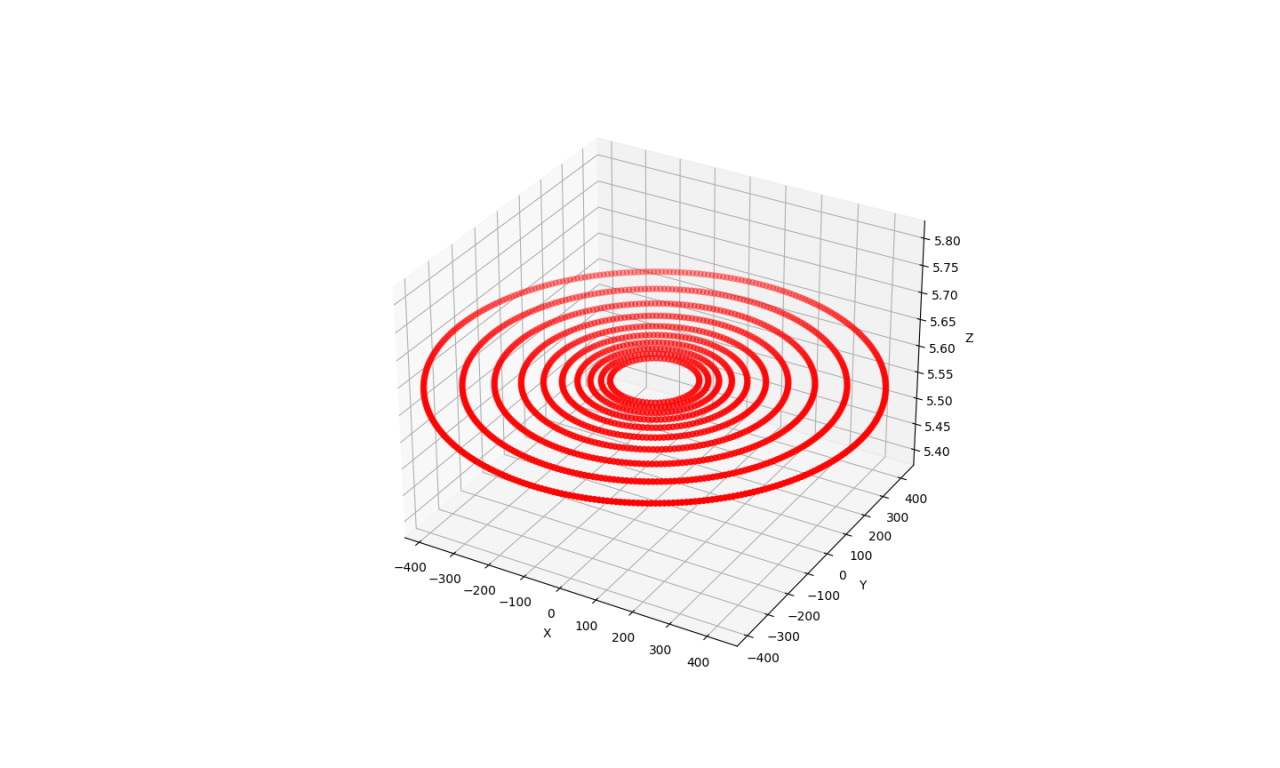
\includegraphics[width=1.0\linewidth]{蚊香.png}  
    \caption{第二问镜场的位置分布示意图}     
    \label{img01}  
\end{figure}

\begin{figure}[H]  
    \centering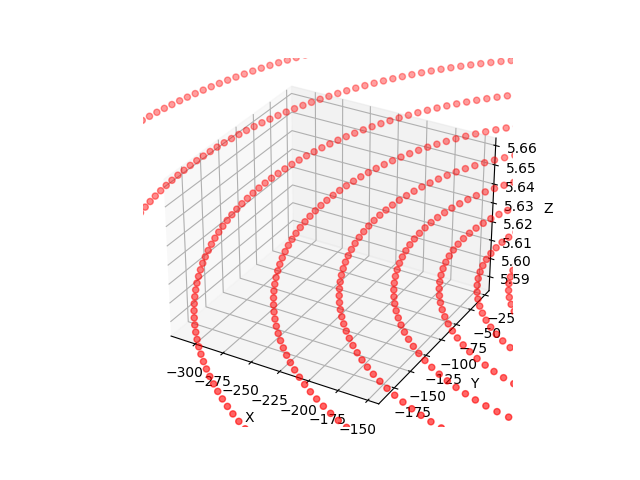
\includegraphics[width=0.6\linewidth]{放大.png}  
    \caption{第二问镜场的位置分布细节示意图}     
    \label{img01}  
\end{figure}


\textbf{2.求解结果如表所示,位置坐标详见附近result2:}

\begin{center}
    \renewcommand{\arraystretch}{1.5}
    \begin{table}[htbp]
        \centering
        \caption{问题二每月21日平均光学效率及输出功率}
        \resizebox{\textwidth}{!}{
          \begin{tabular}{|*{6}{c|}}
            \hline 
            \makecell{日期} & 平均光学效率 & 平均余弦效率 & 平均阴影遮挡效率 & 平均截断效率 & 单位面积镜面平均输出热功率($kw/m^2$) \\
            \hline
            1月21日 &0.698620574 &0.9649707361417448 &0.994760834 &0.955166126 &0.6792664  \\
            \hline
            2月21日 &0.693286145 &0.9532864364541885 &0.996843987 &0.969722613 &0.6501465  \\
            \hline
            3月21日 &0.677196523 &0.9327813457422291 &0.992222965 &0.943604216 &0.6809641  \\
            \hline
            4月21日 &0.650787062 &0.8961058452927791 &0.997682325 &0.990420143 &0.6989222  \\
            \hline
            5月21日 &0.611902191 &0.8631033121094988 &0.974857263 &0.980482644 &0.6780019  \\
            \hline
            6月21日 &0.595230551 &0.852582872076416  &0.950000298 &0.975356811 &0.6687854 \\
            \hline
            7月21日 &0.612444169 &0.8646187195458157 &0.975583334 &0.962305589 &0.6754912  \\
            \hline
            8月21日 &0.651454278 &0.8912604186524585 &0.997344826 &0.990297226 &0.6935248  \\
            \hline
            9月21日 &0.677893281 &0.9309575117008334 &0.984119999 &0.983680421 &0.6812351  \\
            \hline
            10月21日&0.694662874 &0.9531902292611617 &0.994054999 &0.980420143 &0.6523156  \\
            \hline
            11月21日&0.698690764 &0.9617189398583448 &0.994857564 &0.984892644 &0.6156241  \\
            \hline
            12月21日&0.698017600 &0.9616393073744009 &0.990000001 &0.998536811 &0.6543261 \\
            \hline
          \end{tabular}
        }
        \label{tab:example}
      \end{table}
\end{center}

\begin{center}
    \renewcommand{\arraystretch}{1.5}
    \begin{table}[htbp]
        \centering
        \caption{问题二年平均光学效率及输出功率表}
        \resizebox{\textwidth}{!}{
          \begin{tabular}{|*{5}{c|}}
            \hline 
            平均光学效率 & 平均余弦效率 & 平均阴影遮挡效率 & 平均截断效率 & 单位面积镜面平均输出热功率($kw/m^2$) \\
            \hline
            0.663324166 &0.91884667 &0.9868458333 &0.979259666 &0.6690383166  \\
            \hline
          \end{tabular}
        }
        \label{tab:example}
      \end{table}
\end{center}

\begin{table}[H]
    \centering
    \renewcommand{\arraystretch}{1.5}
    \caption{问题二设计参数表}
    \resizebox{\textwidth}{!}{
      \begin{tabular}{|*{5}{c|}}
        \hline 
        吸收塔位置坐标 & 定日镜尺寸(宽*高) & 定日镜安装高度(m) & 定日镜总面数 & 定日镜总面积($m^2$) \\
        \hline
        (0,200,80) & 5*4 &84 &1825 &36500  \\
        \hline
      \end{tabular}
    }
    \label{tab:example}
  \end{table}



% \begin{figure}[H]
%     \centering
%     \subfigure[整体位置示意图]{
%         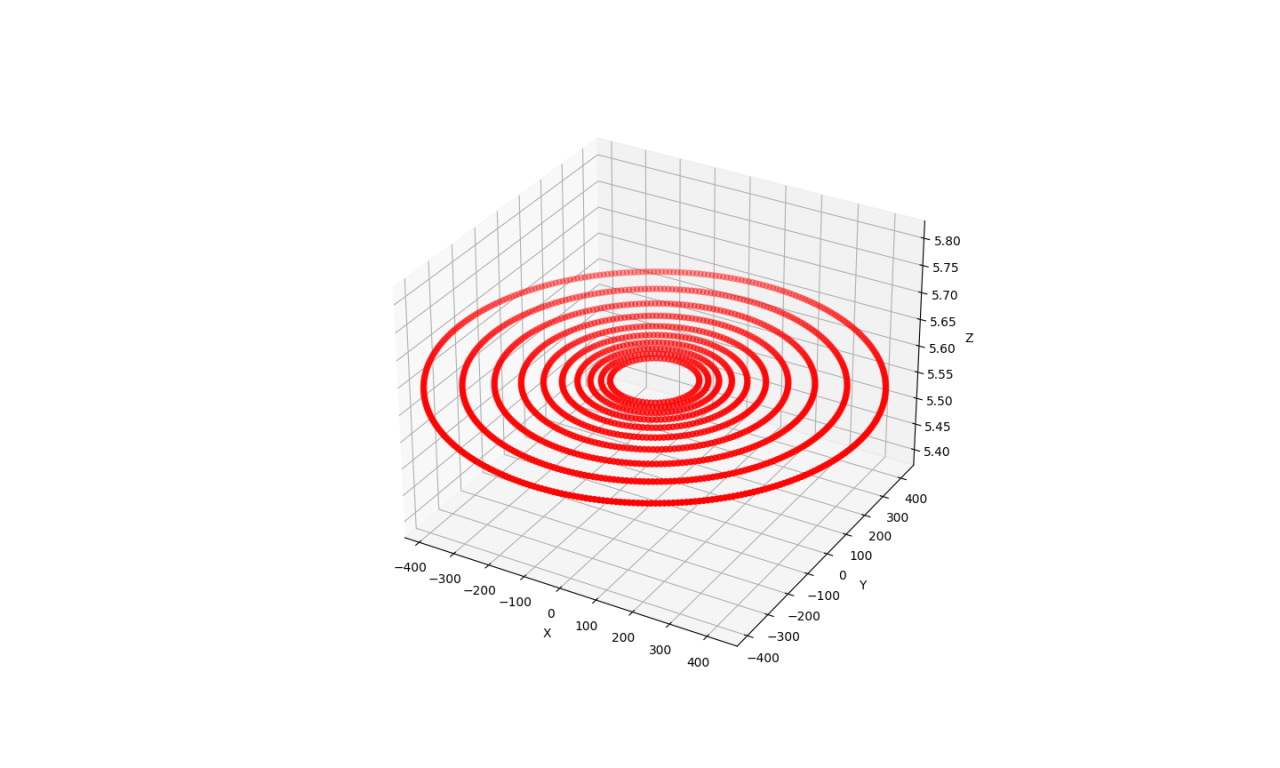
\includegraphics[width=0.8\linewidth]{蚊香.png}
%         \label{fig:img01}
%     }
%     \subfigure[位置示意图]{
%         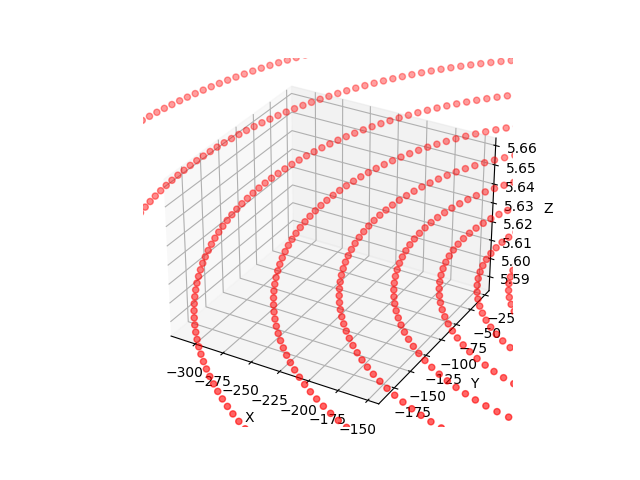
\includegraphics[width=0.4\linewidth]{放大.png}
%         \label{fig:img02}
%     }
%     %\caption{室内温度比较}
%     \label{fig:comparison}
% \end{figure}



\subsection{问题三模型的建立与求解}
\subsubsection{第三问模型的建立}
第三问相较第二问,增加了定日镜的尺寸和高度不同,需要进一步考虑以单位镜面面积年平均输出热功率最大为目标的优化函数模型,
如果考虑各镜的不同尺寸和高度,那么问题的复杂度会大大增加,因此我们考虑将定日镜按位置和效率分为几类,每一类定日镜的尺寸和高度相同,从而简化问题。


% \begin{table}[ht]
%     \centering
%     \caption{示例表格}
%     \begin{tabular}{|c|c|c|c|c|c|}
%     \hline
%     列1 & 列2 & 列3 & 列4 & 列5 & 列6 \\
%     \hline
%     行1 & 数据 & 数据 & 数据 & 数据 & 数据 \\
%     行2 & 数据 & 数据 & 数据 & 数据 & 数据 \\
%     行3 & 数据 & 数据 & 数据 & 数据 & 数据 \\
%     行4 & 数据 & 数据 & 数据 & 数据 & 数据 \\
%     行5 & 数据 & 数据 & 数据 & 数据 & 数据 \\
%     行6 & 数据 & 数据 & 数据 & 数据 & 数据 \\
%     行7 & 数据 & 数据 & 数据 & 数据 & 数据 \\
%     行8 & 数据 & 数据 & 数据 & 数据 & 数据 \\
%     行9 & 数据 & 数据 & 数据 & 数据 & 数据 \\
%     行10 & 数据 & 数据 & 数据 & 数据 & 数据 \\
%     行11 & 数据 & 数据 & 数据 & 数据 & 数据 \\
%     行12 & 数据 & 数据 & 数据 & 数据 & 数据 \\
%     行13 & 数据 & 数据 & 数据 & 数据 & 数据 \\
%     \hline
%     \end{tabular}
%     \end{table}
    

% \begin{center}
%     \renewcommand{\arraystretch}{2.5}
%     \begin{table}[htbp]
%         \centering
%         \caption{问题一每月21日平均光学效率及输出功率}
%         \resizebox{\textwidth}{!}{
%           \begin{tabular}{|*{6}{c|}}
%             \hline
%             \makecell{日期} & 平均光学效率 & 平均余弦效率 & 平均阴影遮挡效率 & 平均截断效率 &单位面积镜面平均输出热功率(kW/m^2)/KWh \\
%             \hline
%             1月21日\textdegree C &12.2965 &42.5769 &55.8333 &23.05589 &46.7999 \\
%             \hline
%             2月21日\textdegree C &13.3751 &32.6129 &47.3448 &29.7226 &59.7333 \\
%             \hline
%             3月21日\textdegree C &14.4168 &36.2857 &41.9999 &36.0421 &72.0000  \\
%             \hline
%             4月21日\textdegree C &16.3515 &23.1667 &40.4999 &42.0143 &83.8666 \\
%             \hline
%             5月21日\textdegree C &18.2896 &20.1081 &39.4857 &48.2644 &96.2666  \\
%             \hline
%             6月21日\textdegree C &20.3423 &18.0000 &39.0000 &53.6811 &106.4000  \\
%             \hline
%           \end{tabular}
%         }
%         \label{tab:example}
%       \end{table}
% % \end{center}
% 在满足温控区间约束条件下,要分析典型房间温变过程微分方程稳态解的性
% 态及模型参数对稳态解变化规律的影响。基于上述的思想建立求解模型,通
% 过使用SIR模型迭代求解常微分方程,从而进行分析。

% 根据题目描述的房间温变过程的集总参数常微分方程为:

% \begin{equation}
%     \begin{cases}
%         C_{in} \frac{d\theta _{in}(t)}{dt}= P_{heat}(t)-\frac{\theta _{in}(t)-\theta _{wall}(t)}{R_{1}}  \\
%         C_{wall} \frac{d\theta _{wall}(t)}{dt}= \frac{\theta _{in}(t)-\theta _{wall}(t)}{R_{1}} -\frac{\theta _{wall}(t)-\theta _{out}(t)}{R_{2}}
%     \end{cases}
% \end{equation}

% \begin{equation}
%     \theta _{in}(0)=\theta _{in0},\theta _{wall}(0)=\theta _{wall0}
% \end{equation}

% 将以上公式通过SIR模型进行转化:

% \begin{equation}
%     \begin{cases}
%         \frac{di(t)}{dt}= \lambda s(t)i(t)-\mu i(t)  \\
%         \frac{ds(t)}{dt}= - \lambda s(t)i(t),t\in [0,T]   \\
%         i(0)=i_0,s(0)=s_0
%     \end{cases}
% \end{equation}

% 从而解出该形式下的数值解格式:

% \begin{equation}
%     \begin{cases}
%         i_{n+1} = i_n + dt(\lambda s_n i_n-\mu i_n)  \\
%         s_{n+1} = s_n - dt \lambda s_n i_n,n=0,1...,N-1   \\
%         i_0,s_0
%     \end{cases}
% \end{equation}

% 从而进行代入题目要求的条件可得:

% \begin{equation}
%     \begin{cases}
%         dT_{in} =  \frac{3600(P_N-(T_{in}-T_{wall}))}{R_1 C_{in}}  \\
%         dT_{wall} = \frac{3600}{c_{wall}} [\frac{(T_{in}-T_{wall})}{R_1}-\frac{(T_{wall}-T_{out})}{R_2}]
%     \end{cases}
% \end{equation}

% 在此过程中,要满足在温控区间的限制,所以温度在18-22之间进行反复跳动,所以我们使用了0-1变量来控制制热器的开关状态。初状态让制热器保持开状态,判断当温度大于22度时,关闭开关,当温度低于18度时,打开开关。进行重复,从而可以得到一个较为稳定的周期变化。

% \subsubsection{第二问模型的求解与结果分析}

% 该模型为简单的微分方程求解问题,但是由于模型参数及数
% 据较多,所以我们将其转换成差分方程迭代求解其数值解。
% 我们使用Pythonscipy中的odeint来进行求解进行求解,结合题意,在满足温控区间的条件
% 下,求解出在一段时间内室内温度和墙体温度的值,来分析微
% 分方程稳态解。使用0-1变量来代表开关状态,从而分析制热功
% 率、室内温度、墙体温度的变化规律,最后依次改变热阻R1、
% 热阻R2、热容及电采暖额定功率结合稳态解来分析等值模型参数
% 对稳态解的影响。

% 最终我们解得答案如图所示:

% \begin{figure}[H]  
%     \centering\includegraphics[width=0.8\linewidth]{室内温度和墙体温度.png}  
%     \caption{室内温度和墙体温度稳态}     
%     \label{img01}  
% \end{figure}

% \begin{figure}[H]  
%     \centering\includegraphics[width=0.8\linewidth]{开关变化.png}  
%     \caption{开关状态图}     
%     \label{img01}  
% \end{figure}

% 由上图分析得,室内温度和墙体温度随时间周期性变化,墙体的温度大致稳定在15.365℃,室内温度在忽略误差的情况下在18℃-22℃以内做周期变化。


% \subsubsection{第二问模型的建立}
% 在满足温控区间约束条件下,要分析典型房间温变过程微分方程稳态解的性
% 态及模型参数对稳态解变化规律的影响。基于上述的思想建立求解模型,通
% 过使用离散欧拉法迭代求解常微分方程,从而进行分析。

% 根据题目描述的房间温变过程的集总参数常微分方程为:

% \begin{equation}
%     \begin{cases}
%         C_{in} \frac{d\theta _{in}(t)}{dt}= P_{heat}(t)-\frac{\theta _{in}(t)-\theta _{wall}(t)}{R_{1}}  \\
%         C_{wall} \frac{d\theta _{wall}(t)}{dt}= \frac{\theta _{in}(t)-\theta _{wall}(t)}{R_{1}} -\frac{\theta _{wall}(t)-\theta _{out}(t)}{R_{2}}
%     \end{cases}
% \end{equation}

% \begin{equation}
%     \theta _{in}(0)=\theta _{in0},\theta _{wall}(0)=\theta _{wall0}
% \end{equation}

% 将以上公式通过离散欧拉法进行转化:

% \begin{equation}
%     y_{n+1} = y_n +h f(x_n,y_n),n=0,1...,N-1
% \end{equation}

% 对区间$[a,b]$进行$N$等分,步长$h=\frac {b-a}{N}$,离散结点为$x_n=a+nh$,$n=0,1...,N$。从而进行代入题目要求的条件

% 设置$s(t)$为0-1变量,代表开关状态,由题意可知,$P_{heat}=s(t)P_N$,代表制热功率,可解出该形式下的数值解格式:
% \begin{equation}
%     \begin{cases}
%         \frac{\theta _{in}(t)}{dt} =  \frac{P_{heat}}{c_{in}}-\frac{\theta_{in}-\theta_{wall}}{R_1 c_{in}}  \\
%         \frac{\theta _{wall}(t)}{dt} =  \frac{\theta_{in}-\theta_{wall}}{c_{wall}R_1}-\frac{\theta_{wall}-\theta_{out}}{R_2 c_{wall}}
%     \end{cases}
% \end{equation}
















% \subsubsection{第二问模型的求解与结果分析}

% 该模型为简单的微分方程求解问题,但是由于模型参数及数
% 据较多,所以我们将其转换成差分方程迭代求解其数值解。
% 我们使用离散欧拉法来进行求解进行求解,结合题意,在满足温控区间的条件
% 下,求解出在一段时间内室内温度和墙体温度的值,使用0-1变量来代表开关状
% 态,从而分析制热功率、室内温度、墙体温度的变化规律,
% 同时,根据室内温度算出总上调时间和总下降时间,利用下一时间节点的
% 室内温度和下一时间节点的室内温度作差,判断是否大于0,若大于0,则证明
% 开关为打开状态,若小于0,则证明是关闭状态。总下降时间反之。

% 根据室内温度上升下降的时间,同时删掉第一个和最后一个时间段,
% 然后将其总时间求平均值,则为周期。利用开关状态为一的时间与
% 总时间进行比例,求出占空比。同时根据使用用电功率和总升温时长
% 求出日用电量和日平均用电功率及用电成本。

% 下面是典型住户电采暖负荷用电行为特征量统计结果:

% \begin{center}
%     \renewcommand{\arraystretch}{2.5}
%     \begin{table}[htbp]
%         \centering
%         \caption{典型住户电采暖负荷用电行为特征量统计结果}
%         \resizebox{\textwidth}{!}{
%           \begin{tabular}{|*{8}{c|}}
%             \hline
%             \makecell{室外\\温度} & 平均升温时长/min & 平均降温时长/min & 周期/min & 平均占空比/\% & 日用电量/KWh&日平均用电功率/kw &日用电成本/元 \\
%             \hline
%             0\textdegree C &12.2965 &42.5769 &55.8333 &23.05589 &46.7999 &1.9499 &19.9888 \\
%             \hline
%             -5\textdegree C &13.3751 &32.6129 &47.3448 &29.7226 &59.7333 &2.4888 &25.5248 \\
%             \hline
%             -10\textdegree C &14.4168 &36.2857 &41.9999 &36.0421 &72.0000 &3.0000 &30.944 \\
%             \hline
%             -15\textdegree C &16.3515 &23.1667 &40.4999 &42.0143 &83.8666 &3.4944 &36.5008 \\
%             \hline
%             -20\textdegree C &18.2896 &20.1081 &39.4857 &48.2644 &96.2666 &4.0111 &41.4928 \\
%             \hline
%             -25\textdegree C &20.3423 &18.0000 &39.0000 &53.6811 &106.4000 &4.4333 &46.2504 \\
%             \hline
%           \end{tabular}
%         }
%         \label{tab:example}
%       \end{table}
% \end{center}

% \begin{figure}[H]
%     \centering
%     \subfigure[室外温度 0度室内温度]{
%         \includegraphics[width=0.4\linewidth]{室内温度0.png}
%         \label{fig:img01}
%     }
%     \subfigure[室外温度 -5度室内温度]{
%         \includegraphics[width=0.4\linewidth]{室内温度-5.png}
%         \label{fig:img02}
%     }
%     %\caption{室内温度比较}
%     \label{fig:comparison}
% \end{figure}

% \begin{figure}[H]
%     \centering
%     \subfigure[室外温度 -10度室内温度]{
%         \includegraphics[width=0.4\linewidth]{室内温度-10.png}
%         \label{fig:img01}
%     }
%     \subfigure[室外温度 -15度室内温度]{
%         \includegraphics[width=0.4\linewidth]{室内温度-15.png}
%         \label{fig:img02}
%     }
%     %\caption{室内温度比较}
%     \label{fig:comparison}
% \end{figure}

% \begin{figure}[H]
%     \centering
%     \subfigure[室外温度 -20度室内温度]{
%         \includegraphics[width=0.4\linewidth]{室内温度-20.png}
%         \label{fig:img01}
%     }
%     \subfigure[室外温度 -25度室内温度]{
%         \includegraphics[width=0.4\linewidth]{室内温度-25.png}
%         \label{fig:img02}
%     }
%     %\caption{室内温度比较}
%     \label{fig:comparison}
% \end{figure}


% 不同温度下设备开关状态如图:
% \begin{figure}[H]
%     \centering
%     \subfigure[室外温度0度电采暖设备开关状态]{
%         \includegraphics[width=0.4\linewidth]{电采暖设备开关状态0.png}
%         \label{fig:img01}
%     }
%     \subfigure[室外温度-5度电采暖设备开关状态]{
%         \includegraphics[width=0.4\linewidth]{电采暖设备开关状态-5.png}
%         \label{fig:img02}
%     }
%     %\caption{室内温度比较}
%     \label{fig:comparison}
% \end{figure}

% \begin{figure}[H]
%     \centering
%     \subfigure[室外温度-10度电采暖设备开关状态]{
%         \includegraphics[width=0.4\linewidth]{电采暖设备开关状态-10.png}
%         \label{fig:img01}
%     }
%     \subfigure[室外温度-15度电采暖设备开关状态]{
%         \includegraphics[width=0.4\linewidth]{电采暖设备开关状态-15.png}
%         \label{fig:img02}
%     }
%     %\caption{室内温度比较}
%     \label{fig:comparison}
% \end{figure}

% \begin{figure}[H]
%     \centering
%     \subfigure[室外温度-20度电采暖设备开关状态]{
%         \includegraphics[width=0.4\linewidth]{电采暖设备开关状态-20.png}
%         \label{fig:img01}
%     }
%     \subfigure[室外温度-25度电采暖设备开关状态]{
%         \includegraphics[width=0.4\linewidth]{电采暖设备开关状态-25.png}
%         \label{fig:img02}
%     }
%     %\caption{室内温度比较}
%     \label{fig:comparison}
% \end{figure}

% 不同温度下设备开关状态如图:
% \begin{figure}[H]
%     \centering
%     \subfigure[墙体温度 0度]{
%         \includegraphics[width=0.4\linewidth]{墙体温度0.png}
%         \label{fig:img01}
%     }
%     \subfigure[墙体温度-5度]{
%         \includegraphics[width=0.4\linewidth]{墙体温度-5.png}
%         \label{fig:img02}
%     }
%     %\caption{室内温度比较}
%     \label{fig:comparison}
% \end{figure}

% \begin{figure}[H]
%     \centering
%     \subfigure[墙体温度 -10度]{
%         \includegraphics[width=0.4\linewidth]{墙体温度-10.png}
%         \label{fig:img01}
%     }
%     \subfigure[墙体温度-15度]{
%         \includegraphics[width=0.4\linewidth]{墙体温度-15.png}
%         \label{fig:img02}
%     }
%     %\caption{室内温度比较}
%     \label{fig:comparison}
% \end{figure}

% \begin{figure}[H]
%     \centering
%     \subfigure[墙体温度 -20度]{
%         \includegraphics[width=0.4\linewidth]{墙体温度-20.png}
%         \label{fig:img01}
%     }
%     \subfigure[墙体温度-25度]{
%         \includegraphics[width=0.4\linewidth]{墙体温度-25.png}
%         \label{fig:img02}
%     }
%     %\caption{室内温度比较}
%     \label{fig:comparison}
% \end{figure}

% 结合表格数据与图形分析可得,室外温度越低,设备平均升温时长越长,降温时长越短,
% 周期越短,用电量也越大。


% \subsubsection{第三问模型的建立}

% 第三问要计算供暖期典型住户用电量和用电成本,基于第二问的模型基础上,
% 分别对180天分段进行计算,得到每个时段需要的数据。


% \subsubsection{第三问模型的求解与结果分析}

% 利用第二题建立的模型与公式,进行计算可得到供暖期典型住户用电量
% 和用电成本统计结果:

% \begin{center}
%     %\renewcommand{\arraystretch}{2.5}
%     \begin{table}[htbp]
%         \centering
%         \caption{供暖期典型住户用电量和用电成本统计结果}
%           \begin{tabular}{|p{4cm}|p{4cm}|p{4cm}|p{4cm}|}
%             \hline
%             室外平均温度 & 持续天数 & 用电量/Kwh & 供暖成本/元  \\
%             \hline
%             0\textdegree C &30 &1403.997 &599.664  \\
%             \hline
%             -5\textdegree C &40 &2389.332 &1020.992 \\
%             \hline
%             -10\textdegree C &40 &2880.000 &1237.76 \\
%             \hline
%             -15\textdegree C &40 &3354.640 &1460.032 \\
%             \hline
%             -20\textdegree C &30 &2887.998 &1244.784 \\
%             \hline
%           \end{tabular}
%         \label{tab:example}
%       \end{table}
% \end{center}
% 供暖期总用电量:12915.967/Kwh,供暖期总成本:5563.232/元。


% \subsection{问题二}
% \subsubsection{第一问模型的建立}
% 在满足温控区间约束条件下,要分析典型房间温变过程微分方程稳态解的性态及模
% 型参数对稳态解变化规律的影响。基于问题一的思想建立求解模型,通过使用离散欧拉法
% 迭代求解常微分方程,从而进行分析。

% \subsubsection{第一问模型的求解与结果分析}

% \begin{figure}[H]  
%     \centering\includegraphics[width=0.8\linewidth]{室外温度-15上下调可持续时间.png}  
%     \caption{室外温度-15度上下调可持续时间}     
%     \label{img01}  
% \end{figure}

% 如果该点正处于电采暖设备开启状态,即所对应的值为上调的可持续时间,反之则为下调可持续时间。


% \subsubsection{第二问模型的求解与结果分析}

% \begin{figure}[H]
%     \centering
%     \subfigure[室外温度0度上下调可持续时间]{
%         \includegraphics[width=0.4\linewidth]{室外温度0上下调可持续时间.png}
%         \label{fig:img01}
%     }
%     \subfigure[室外温度-5度上下调可持续时间]{
%         \includegraphics[width=0.4\linewidth]{室外温度-5上下调可持续时间.png}
%         \label{fig:img02}
%     }
%     %\caption{室内温度比较}
%     \label{fig:comparison}
% \end{figure}


% \begin{figure}[H]
%     \centering
%     \subfigure[室外温度-10度上下调可持续时间]{
%         \includegraphics[width=0.4\linewidth]{室外温度-10上下调可持续时间.png}
%         \label{fig:img01}
%     }
%     \subfigure[室外温度-15度上下调可持续时间]{
%         \includegraphics[width=0.4\linewidth]{室外温度-15上下调可持续时间.png}
%         \label{fig:img02}
%     }
%     %\caption{室内温度比较}
%     \label{fig:comparison}
% \end{figure}

% \begin{figure}[H]
%     \centering
%     \subfigure[室外温度-20度上下调可持续时间]{
%         \includegraphics[width=0.4\linewidth]{室外温度-20上下调可持续时间.png}
%         \label{fig:img01}
%     }
%     \subfigure[室外温度-25度上下调可持续时间]{
%         \includegraphics[width=0.4\linewidth]{室外温度-25上下调可持续时间.png}
%         \label{fig:img02}
%     }
%     %\caption{室内温度比较}
%     \label{fig:comparison}
% \end{figure}

% 由图分析可得,随着室外温度的降低,上调可持续时间逐渐增加,下调可持续时间逐渐减少。


% \subsection{问题三}
% \subsubsection{第一问模型的建立}

% 在设定开关为开的前提下,将 6 个住户的室内初始温度设定在在温控区间 18℃-
% 20℃ 内均匀分布,墙体温度初始化为可以使得墙体的处于平衡状态时的温度,墙体对
% 外的输出能量等于墙体室内温度对墙的输入能量,能量守恒墙体温度恒定不变。根据集
% 总参数微分方程中的第一个等式,通过迭代法计算每个时刻住宅区各个住户的室内温度
% 随时间的变化结果,并记录下开关的状态,得到每个住户的用电功率曲线,将上述内容
% 重复 6 次,得到 6 个住户的总用电功率曲线。

% \subsubsection{第一问模型的求解与结果分析}

% 24小时室内温度变化图:
% \begin{figure}[H]
%     \centering
%     \subfigure[1号室内温度]{
%         \includegraphics[width=0.4\linewidth]{1号室内温度-20.png}
%         \label{fig:img01}
%     }
%     \subfigure[2号室内温度]{
%         \includegraphics[width=0.4\linewidth]{2号室内温度-20.png}
%         \label{fig:img02}
%     }
%     %\caption{室内温度比较}
%     \label{fig:comparison}
% \end{figure}

% \begin{figure}[H]
%     \centering
%     \subfigure[3号室内温度]{
%         \includegraphics[width=0.4\linewidth]{3号室内温度-20.png}
%         \label{fig:img01}
%     }
%     \subfigure[4号室内温度]{
%         \includegraphics[width=0.4\linewidth]{4号室内温度-20.png}
%         \label{fig:img02}
%     }
%     %\caption{室内温度比较}
%     \label{fig:comparison}
% \end{figure}

% \begin{figure}[H]
%     \centering
%     \subfigure[5号室内温度]{
%         \includegraphics[width=0.4\linewidth]{5号室内温度-20.png}
%         \label{fig:img01}
%     }
%     \subfigure[6号室内温度]{
%         \includegraphics[width=0.4\linewidth]{6号室内温度-20.png}
%         \label{fig:img02}
%     }
%     %\caption{室内温度比较}
%     \label{fig:comparison}
% \end{figure}

% 24小时电采暖设备的开关状态变化图:
% \begin{figure}[H]
%     \centering
%     \subfigure[1号开关状态]{
%         \includegraphics[width=0.4\linewidth]{1号开关状态-20.png}
%         \label{fig:img01}
%     }
%     \subfigure[2号开关状态]{
%         \includegraphics[width=0.4\linewidth]{2号开关状态-20.png}
%         \label{fig:img02}
%     }
%     %\caption{室内温度比较}
%     \label{fig:comparison}
% \end{figure}

% \begin{figure}[H]
%     \centering
%     \subfigure[3号开关状态]{
%         \includegraphics[width=0.4\linewidth]{3号开关状态-20.png}
%         \label{fig:img01}
%     }
%     \subfigure[4号开关状态]{
%         \includegraphics[width=0.4\linewidth]{4号开关状态-20.png}
%         \label{fig:img02}
%     }
%     %\caption{室内温度比较}
%     \label{fig:comparison}
% \end{figure}

% \begin{figure}[H]
%     \centering
%     \subfigure[5号开关状态]{
%         \includegraphics[width=0.4\linewidth]{5号开关状态-20.png}
%         \label{fig:img01}
%     }
%     \subfigure[6号开关状态]{
%         \includegraphics[width=0.4\linewidth]{6号开关状态-20.png}
%         \label{fig:img02}
%     }
%     %\caption{室内温度比较}
%     \label{fig:comparison}
% \end{figure}

% 6个住户的总用电功率曲线:

% \begin{figure}[H]  
%     \centering\includegraphics[width=0.8\linewidth]{总功率-20.png}  
%     \caption{6个住户的总用电功率曲线}     
%     \label{img01}  
% \end{figure}

% 在每一时段6个住户用电功率相加,一开始由于开启状态,所以总用电功率较高,后面逐渐稳定。

% \subsubsection{第二问模型的求解与结果分析}

% 以上述6个住户总用电功率曲线为基础,24小时各时点总可上调、下调功率:
% \begin{figure}[H]
%     \centering
%     \subfigure[1号上下调功率]{
%         \includegraphics[width=0.4\linewidth]{1号室外温度-20上下调可持续时间.png}
%         \label{fig:img01}
%     }
%     \subfigure[2号上下调功率]{
%         \includegraphics[width=0.4\linewidth]{2号室外温度-20上下调可持续时间.png}
%         \label{fig:img02}
%     }
%     %\caption{室内温度比较}
%     \label{fig:comparison}
% \end{figure}

% \begin{figure}[H]
%     \centering
%     \subfigure[3号上下调功率]{
%         \includegraphics[width=0.4\linewidth]{3号室外温度-20上下调可持续时间.png}
%         \label{fig:img01}
%     }
%     \subfigure[4号上下调功率]{
%         \includegraphics[width=0.4\linewidth]{4号室外温度-20上下调可持续时间.png}
%         \label{fig:img02}
%     }
%     %\caption{室内温度比较}
%     \label{fig:comparison}
% \end{figure}

% \begin{figure}[H]
%     \centering
%     \subfigure[5号上下调功率]{
%         \includegraphics[width=0.4\linewidth]{5号室外温度-20上下调可持续时间.png}
%         \label{fig:img01}
%     }
%     \subfigure[6号上下调功率]{
%         \includegraphics[width=0.4\linewidth]{6号室外温度-20上下调可持续时间.png}
%         \label{fig:img02}
%     }
%     %\caption{室内温度比较}
%     \label{fig:comparison}
% \end{figure}


% \subsubsection{第三问模型的求解与结果分析}
% 各室外温度下,电采暖设备可调节能力:
% \begin{figure}[H]
%     \centering
%     \subfigure[0度总可上下调功率]{
%         \includegraphics[width=0.4\linewidth]{室外温度0总可上下调功率.png}
%         \label{fig:img01}
%     }
%     \subfigure[-5度总可上下调功率]{
%         \includegraphics[width=0.4\linewidth]{室外温度-5总可上下调功率.png}
%         \label{fig:img02}
%     }
%     %\caption{室内温度比较}
%     \label{fig:comparison}
% \end{figure}

% \begin{figure}[H]
%     \centering
%     \subfigure[-10度总可上下调功率]{
%         \includegraphics[width=0.4\linewidth]{室外温度-10总可上下调功率.png}
%         \label{fig:img01}
%     }
%     \subfigure[-15度总可上下调功率]{
%         \includegraphics[width=0.4\linewidth]{室外温度-15总可上下调功率.png}
%         \label{fig:img02}
%     }
%     %\caption{室内温度比较}
%     \label{fig:comparison}
% \end{figure}

% \begin{figure}[H]
%     \centering
%     \subfigure[-20度总可上下调功率]{
%         \includegraphics[width=0.4\linewidth]{室外温度-20总可上下调功率.png}
%         \label{fig:img01}
%     }
%     \subfigure[-25度总可上下调功率]{
%         \includegraphics[width=0.4\linewidth]{室外温度-25总可上下调功率.png}
%         \label{fig:img02}
%     }
%     %\caption{室内温度比较}
%     \label{fig:comparison}
% \end{figure}

% 由图分析可得,随着室外温度不断下降,多个电采暖负荷的调节能力也逐渐下降。

% \subsection{问题四}

% \subsubsection{模型的求解与结果分析}

% 600住户总可上下调功率图:
% \begin{figure}[H]
%     \centering
%     \subfigure[600住户0度总可上下调功率]{
%         \includegraphics[width=0.4\linewidth]{6室外温度0总可上下调功率.png}
%         \label{fig:img01}
%     }
%     \subfigure[600住户-5度总可上下调功率]{
%         \includegraphics[width=0.4\linewidth]{6室外温度-5总可上下调功率.png}
%         \label{fig:img02}
%     }
%     %\caption{室内温度比较}
%     \label{fig:comparison}
% \end{figure}

% \begin{figure}[H]
%     \centering
%     \subfigure[600住户-10度总可上下调功率]{
%         \includegraphics[width=0.4\linewidth]{6室外温度-10总可上下调功率.png}
%         \label{fig:img01}
%     }
%     \subfigure[600住户-15度总可上下调功率]{
%         \includegraphics[width=0.4\linewidth]{6室外温度-15总可上下调功率.png}
%         \label{fig:img02}
%     }
%     %\caption{室内温度比较}
%     \label{fig:comparison}
% \end{figure}

% \begin{figure}[H]
%     \centering
%     \subfigure[600住户-20度总可上下调功率]{
%         \includegraphics[width=0.4\linewidth]{6室外温度-20总可上下调功率.png}
%         \label{fig:img01}
%     }
%     \subfigure[600住户-25度总可上下调功率]{
%         \includegraphics[width=0.4\linewidth]{6室外温度-25总可上下调功率.png}
%         \label{fig:img02}
%     }
%     %\caption{室内温度比较}
%     \label{fig:comparison}
% \end{figure}


% 600住户总功率图:
% \begin{figure}[H]
%     \centering
%     \subfigure[600住户0度总功率]{
%         \includegraphics[width=0.4\linewidth]{6总功率0.png}
%         \label{fig:img01}
%     }
%     \subfigure[600住户-5度总功率]{
%         \includegraphics[width=0.4\linewidth]{6总功率-5.png}
%         \label{fig:img02}
%     }
%     %\caption{室内温度比较}
%     \label{fig:comparison}
% \end{figure}

% \begin{figure}[H]
%     \centering
%     \subfigure[600住户-10度总功率]{
%         \includegraphics[width=0.4\linewidth]{6总功率-10.png}
%         \label{fig:img01}
%     }
%     \subfigure[600住户-15度总功率]{
%         \includegraphics[width=0.4\linewidth]{6总功率-15.png}
%         \label{fig:img02}
%     }
%     %\caption{室内温度比较}
%     \label{fig:comparison}
% \end{figure}

% \begin{figure}[H]
%     \centering
%     \subfigure[600住户-20度总功率]{
%         \includegraphics[width=0.4\linewidth]{6总功率-20.png}
%         \label{fig:img01}
%     }
%     \subfigure[600住户-25度总功率]{
%         \includegraphics[width=0.4\linewidth]{6总功率-25.png}
%         \label{fig:img02}
%     }
%     %\caption{室内温度比较}
%     \label{fig:comparison}
% \end{figure}

% \subsection{问题五}


% \subsection{问题六}
% \subsubsection{第一问}
% 针对面积为4000万平方米的省级区域电采暖负荷参与电网调节的潜能和可能遇到的问题,可以提出一下分析和展望。

% 潜能:电采暖负荷参与电网调节具有很强的潜能。随着环境问题日益增大,电力系统中可再生能源占比越来越大,其中的不稳定性和间歇性问题也逐渐突出。此时,引入可控、可调电采暖负荷是一个很好的选择。例如,乌鲁木齐今年累计改造改造供暖面积146.15万平方米。据统计,目前乌鲁木齐电采暖面积达到近1500万平方米。它可以通过灵活的调度,实现电力系统的平衡。并且,电采暖负荷可以利用低谷价格,降低用电费用。

% 可能遇到的问题:虽然电采暖负荷参与电网调节具有巨大的潜力,但仍有些不足。首先,电采暖负荷参与调节需要大量的数据支持,因此需要消耗大量的人力物力,以及愿意支持的居民用户。其次,电采暖负荷调节还需要住户的个人意愿,固定的温控区间难以满足每位住户的需求、接入难度大等问题。

% 建议和解决方法:采取适量的奖励机制,增加补偿价格,提高民众意愿度。在网上加大对电采暖政策的宣传力度,开通快速电采暖线上报装服务,满足用户的低碳用能需求。
% \subsubsection{第二问}
% 特点:使用时间段密集,容易形成高峰负荷。室外温度过高,空调负荷波动较大,容易对电网产生影响。

% 潜能:在夏季由于天气因素,空调使用规模非常大,如果可以实现对空调负荷实现可调节,将会有巨大的经济收益以及电量节省,有助于低碳发展的进行。

% 可能遇到的问题:可调节空调难以完全替代老旧空调;对于大量的居宅区进行智能管控,需要巨大的计算能力,可能会受到设备的限制;居民的主观因素影响对新事物的接受度低;智能管控技术不够成熟,可能会造成安全隐患,容易引发智能空调的失控导致财产损失。


\section{模型分析}

\subsection{模型检验}
\textbf{1.余弦效率检验:}

对于特定时刻,我们可以确定太阳的高度角,
进而建立简单几何模型估计余弦效率。
譬如当正午太阳直射时,定光镜倾斜反射太阳
光至集热器,入射光线与吸收塔平行,可由塔
高与镜塔长度推测出$tan(2\theta)$的范围,
进而推测出$cos(\theta)$即余弦效率的范围
,应在0.77至0.91间。

\section{模型总结}
\subsection{模型优点}
模型基于严谨的理论基础推导,基于坐标变换得出了精准的定日镜坐标和各向量,考虑了定日镜场中各因素的影响;

可以根据不同的坐标系选择和转换,灵活地建立定日镜-集热器光线模型,方便地进行光线追踪和反射计算;

可以最大化单位镜面面积年平均输出热功率,同时考虑了额定功率和定日镜要求的约束条件,实现了镜场的优化设计;
\subsection{模型缺点}
模型在计算损失效率为减少计算量时做了许多近似处理,比如忽略了光束发散问题,忽略了太阳高度角对反射太阳光的影响;

模型没有考虑定日镜场的实际情况,比如定日镜场的地形、气候、季节、时间等对效率的影响;

基于python编程,需要大量的计算资源和时间,可能不适合实时或在线的应用场景;


\section{参考文献}

\noindent[1]刘建兴.塔式光热电站光学效率建模仿真及定日镜场优化布置[D].兰州交通大学,2022

\noindent[2]许芬.塔式太阳能定日镜聚光成像建模及仿真[J].太阳能学报,2010,(10): 1304-1310

\noindent[3]郭铁铮,刘德有,钱艳平,陈强,卞新高,郭苏.塔式太阳能热发电站中的定日镜跟踪装置研制[J].中国电机工程学报,2008,第28卷(35): 114-119

\noindent[4]张平等,太阳能塔式光热镜场光学效率计算方法[J],技术与市场,2021,28(6):5-8.

\section{附录}
\subsection{第一题代码}
\inputminted[
    frame=lines,
    framesep=2mm,
    baselinestretch=1.2,
    fontsize=\small,
    linenos
]{python}{code/p1.py}

\subsection{第二题代码}
\inputminted[
    frame=lines,
    framesep=2mm,
    baselinestretch=1.2,
    fontsize=\small,
    linenos
]{python}{code/p1_output.py}

\subsection{第三题第一问代码}
\inputminted[
    frame=lines,
    framesep=2mm,
    baselinestretch=1.2,
    fontsize=\small,
    linenos
]{python}{code/p2.py}

\end{document}




